\section{線形結合と線形独立・従属} \setcounter{ex}{0}

これまでの章では、具体的な数の並びとしてのベクトルとその計算、そして行列の基本的な性質を学びました。これらは線形代数の「計算」の基盤です。この章では、これらの計算が成り立つ「舞台」である\emph{ベクトル空間}について定義し、その上で線形代数の「考え方」の核心に迫る概念である\emph{線形結合}、そしてそれに続く\emph{線形独立}と\emph{線形従属}を深掘りします。

\subsection{ベクトル空間の定義}

\emph{ベクトル空間}は、数学において特定の性質を満たすベクトルの集合のことです。線形代数の概念が成り立つ「舞台」となります。

\begin{dfn}[ベクトル空間] \label{vector_space}
集合 $V$ が\emph{ベクトル空間(または線形空間)である}とは、以下の条件を満たすときに言います。
\begin{enumerate}
\item $V$ の任意の2つの要素(ベクトル)$\bm{u}, \bm{v}$ に対して、和 $\bm{u} + \bm{v}$ が定義されており、その結果も $V$ の要素である。($V$ は\emph{加法について閉じている})
\item $V$ の任意の要素(ベクトル)$\bm{u}$ と、実数(スカラー)$k$ に対して、スカラー倍 $k\bm{u}$ が定義されており、その結果も $V$ の要素である。($V$ は\emph{スカラー倍について閉じている})
\end{enumerate}
さらに、これらの演算が以下の8つの\emph{公理}を満たさなければなりません。\\
\emph{加法に関する公理}:
\begin{itemize}
\item[(A1)] \emph{交換法則}: $\bm{u} + \bm{v} = \bm{v} + \bm{u}$
\item[(A2)] \emph{結合法則}: $(\bm{u} + \bm{v}) + \bm{w} = \bm{u} + (\bm{v} + \bm{w})$
\item[(A3)] \emph{零ベクトルの存在}: $V$ の任意の要素 $\bm{u}$ に対して、$\bm{u} + \bm{0} = \bm{u}$ となる要素 $\bm{0}$(零ベクトル)が $V$ の中に存在する。
\item[(A4)] \emph{逆ベクトルの存在}: $V$ の任意の要素 $\bm{u}$ に対して、$\bm{u} + (-\bm{u}) = \bm{0}$ となる要素 $-\bm{u}$(逆ベクトル)が $V$ の中に存在する。
\end{itemize}
\emph{スカラー倍に関する公理}:
\begin{itemize}
\item[(S1)] \emph{結合法則}: $k(l\bm{u}) = (kl)\bm{u}$
\item[(S2)] \emph{分配法則(スカラーについて)}: $(k+l)\bm{u} = k\bm{u} + l\bm{u}$
\item[(S3)] \emph{分配法則(ベクトルについて)}: $k(\bm{u}+\bm{v}) = k\bm{u} + k\bm{v}$
\item[(S4)] \emph{単位元}: $1\bm{u} = \bm{u}$ (ここで $1$ は実数 $1$)
\end{itemize}
\end{dfn}

\begin{ex}
\begin{itemize}
\item \emph{$n$次元ユークリッド空間 $\mathbb{R}^n$}: これまで扱ってきた数の羅列の集合は、これらの公理を全て満たすため、最も基本的なベクトル空間です。
\item \emph{多項式の集合}: 例えば、2次以下の多項式 $P(x) = ax^2 + bx + c$ 全体の集合もベクトル空間になります。
\item \emph{行列の集合}: 例えば、$2 \times 2$ 行列全体の集合もベクトル空間です。
\end{itemize}
\end{ex}

\subsection{線形結合}

線形結合は、複数のベクトルを足し合わせたり、スカラー倍したりする操作を組み合わせたものです。これまでに学んだベクトルの基本演算の応用と言えます。

\begin{dfn}[線形結合] \label{linear_combination}
$n$次元ベクトル $\bm{v}_1, \bm{v}_2, \ldots, \bm{v}_k$ と、スカラー $c_1, c_2, \ldots, c_k$ が与えられたとき、これらのベクトルとスカラーを用いて作られる以下の式を、\emph{線形結合}と呼びます。
\[c_1 \bm{v}_1 + c_2 \bm{v}_2 + \dots + c_k \bm{v}_k\]
\end{dfn}

\begin{ex}
2つのベクトル $\bm{v}_1 = \begin{pmatrix} 1 \\ 2 \end{pmatrix}$ と $\bm{v}_2 = \begin{pmatrix} 3 \\ 1 \end{pmatrix}$ を考えます。スカラー $c_1 = 2,\ c_2 = -1$ を用いた線形結合は、
\[2\bm{v}_1 + (-1)\bm{v}_2 = 2\begin{pmatrix} 1 \\ 2 \end{pmatrix} - \begin{pmatrix} 3 \\ 1 \end{pmatrix} = \begin{pmatrix} 2 \\ 4 \end{pmatrix} - \begin{pmatrix} 3 \\ 1 \end{pmatrix} = \begin{pmatrix} -1 \\ 3 \end{pmatrix}\]
となります。
\end{ex}

\begin{dfn}[生成する空間 / 線形包] \label{linear_span}
ベクトルの集合 $S = \{ \bm{v}_1, \bm{v}_2, \ldots, \bm{v}_k \}$ のすべての可能な線形結合によって形成されるベクトル全体の集合を、$S$ によって\emph{生成される空間}と呼び、$\text{span}(S)$ または $\text{span}\{\bm{v}_1, \ldots, \bm{v}_k\}$ と表記します。これは\emph{線形包}とも呼ばれます。
\end{dfn}

\emph{幾何学的解釈}:
\begin{itemize}
\item 1つの零ベクトルでないベクトル $\bm{v}_1$ の線形結合 $c_1 \bm{v}_1$ は、原点を通る直線を表します。
\begin{center}
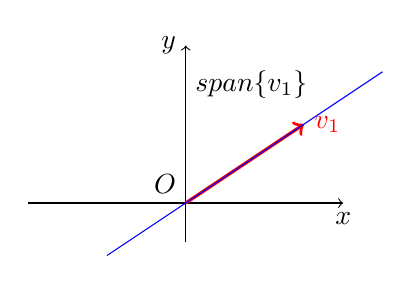
\begin{tikzpicture}
    \draw[->] (-2,0) -- (2,0) node[below] {$x$};
    \draw[->] (0,-0.5) -- (0,2) node[left] {$y$};
    \draw[very thick, red, ->] (0,0) -- (1.5,1) node[right] {$\bm{v}_1$};
    \draw[blue] (-1,-1*1/1.5) -- (2.5,2.5*1/1.5); % 直線 (c_1 v_1)
    \node at (0,0) [above left] {$O$};
    \node at (0,1.5) [right] {$\text{span}\{\bm{v}_1\}$};
\end{tikzpicture}
\end{center}
\item 2つの平行でない零ベクトルでないベクトル $\bm{v}_1, \bm{v}_2$ の線形結合 $c_1 \bm{v}_1 + c_2 \bm{v}_2$ は、原点を通る平面を表します。
\begin{center}
\begin{tikzpicture}
    \fill[blue!10, opacity=0.5] (-2,-1) -- (2,-1) -- (2,1) -- (-2,1) -- cycle; % 平面を表現
    \draw[dashed] (-2,-1) -- (2,-1);
    \draw[dashed] (-2,1) -- (2,1);
    \draw[dashed] (-2,-1) -- (-2,1);
    \draw[dashed] (2,-1) -- (2,1);
    \draw[->] (0,0) -- (1.5,0.5) node[right] {$\bm{v}_1$};
    \draw[->] (0,0) -- (-0.5,1.5) node[above left] {$\bm{v}_2$};
    \node at (0,0) [below left] {$O$};
    \node at (1.5,1.5) [above right] {$\text{span}\{\bm{v}_1, \bm{v}_2\}$ (平面)};
\end{tikzpicture}
\end{center}
\end{itemize}

\begin{ex}
$\bm{v}_1 = \begin{pmatrix} 1 \\ 0 \end{pmatrix}$ と $\bm{v}_2 = \begin{pmatrix} 0 \\ 1 \end{pmatrix}$ によって生成される空間 $\text{span}\{\bm{v}_1, \bm{v}_2\}$ は、2次元平面上のすべてのベクトルを表現できます。これは、任意のベクトル $\begin{pmatrix} x \\ y \end{pmatrix}$ を $x\begin{pmatrix} 1 \\ 0 \end{pmatrix} + y\begin{pmatrix} 0 \\ 1 \end{pmatrix}$ と書けるからです。
\end{ex}

\subsection{線形独立と線形従属}

線形結合の概念を用いることで、ベクトルの集合が持つ「冗長性」を数学的に定義できます。これが\emph{線形独立}と\emph{線形従属}の概念です。

\begin{dfn}[線形独立] \label{linear_independence}
ベクトルの集合 $\{\bm{v}_1, \bm{v}_2, \ldots, \bm{v}_k\}$ が\emph{線形独立である}とは、以下の条件を満たすときに言います。
\[c_1 \bm{v}_1 + c_2 \bm{v}_2 + \dots + c_k \bm{v}_k = \bm{0}\text{ ならば }\forall i.c_i=0\]
\end{dfn}

\begin{dfn}[線形従属] \label{linear_dependence}
ベクトルの集合 $\{\bm{v}_1, \bm{v}_2, \ldots, \bm{v}_k\}$ が\emph{線形従属である}とは、線形独立ではない、つまり,以下の条件を満たすときに言います。
\[c_1 \bm{v}_1 + c_2 \bm{v}_2 + \dots + c_k \bm{v}_k = \bm{0}\text{ かつ }\exists i. c_i\neq0\]
\end{dfn}

\emph{幾何学的解釈}:
\begin{itemize}
\item \emph{線形独立}: どのベクトルも、他のベクトルの線形結合で表せない(つまり、集合内のベクトルがそれぞれ新しい「方向」を持っている)。
\item \emph{線形従属}: 少なくとも1つのベクトルが、他のベクトルの線形結合で表せる(つまり、集合内のベクトルに「冗長性」がある)。例えば、2つのベクトルが線形従属なら、それらは平行です。3つのベクトルが線形従属なら、それらは同一平面上にあるか、あるいは互いに平行です。
\end{itemize}

\begin{thm}[線形従属の判定条件] \label{criteria_for_linear_dependence}
ベクトルの集合 $\{\bm{v}_1, \bm{v}_2, \ldots, \bm{v}_k\}$ が線形従属であることと、集合内の少なくとも1つのベクトルが他のベクトルの線形結合で表せることは同値である。
\begin{proof*}
\begin{itemize}
	\item \emph{($\Rightarrow$) 線形従属ならば、少なくとも1つのベクトルが他のベクトルの線形結合で表せることの証明}:\\
    集合が線形従属であると仮定します。定義\ref{linear_dependence}より、
    \[c_1 \bm{v}_1 + c_2 \bm{v}_2 + \dots + c_k \bm{v}_k = \bm{0}\text{ かつ }\exists i. c_i\neq0\]
    が成り立つようなスカラー $c_1, \ldots, c_k$ が存在します。このとき、少なくとも1つの $c_m \neq 0$ である $m$ が存在します。その $c_m \bm{v}_m$ の項を左辺に残し、他の項を右辺に移項すると、
    \[c_m \bm{v}_m = -c_1 \bm{v}_1 - \dots - c_{m-1} \bm{v}_{m-1} - c_{m+1} \bm{v}_{m+1} - \dots - c_k \bm{v}_k\]
    $c_m \neq 0$ なので、両辺を $c_m$ で割ることができます。
    \[\bm{v}_m = -\frac{c_1}{c_m} \bm{v}_1 - \dots - \frac{c_{m-1}}{c_m} \bm{v}_{m-1} - \frac{c_{m+1}}{c_m} \bm{v}_{m+1} - \dots - \frac{c_k}{c_m} \bm{v}_k\]
    これは、$\bm{v}_m$ が他のベクトル $\{\bm{v}_1, \ldots, \bm{v}_{m-1}, \bm{v}_{m+1}, \ldots, \bm{v}_k\}$ の線形結合で表せることを示しています。
	\item \emph{($\Leftarrow$) 少なくとも1つのベクトルが他のベクトルの線形結合で表せるならば、線形従属であることの証明}:\\
	集合内の少なくとも1つのベクトル、例えば $\bm{v}_m$ が、他のベクトルの線形結合で表せると仮定します。
    \[\bm{v}_m = d_1 \bm{v}_1 + \dots + d_{m-1} \bm{v}_{m-1} + d_{m+1} \bm{v}_{m+1} + \dots + d_k \bm{v}_k\]
    ここで $d_i$ はスカラーです。この式を移項すると、
    \[d_1 \bm{v}_1 + \dots + d_{m-1} \bm{v}_{m-1} + (-1)\bm{v}_m + d_{m+1} \bm{v}_{m+1} + \dots + d_k \bm{v}_k = \bm{0}\]
    この線形結合において、$\bm{v}_m$ の係数は $-1$ であり、$0$ ではありません。したがって、定義\ref{linear_dependence}により、このベクトルの集合は線形従属であると言えます。
\end{itemize}
(証明終)
\end{proof*}
\end{thm}

\begin{ex}[線形独立・従属の判定]
\begin{enumerate}
\item \emph{線形独立の例}:\\
    \[\bm{v}_1 = \begin{pmatrix} 1 \\ 0 \end{pmatrix},\ \bm{v}_2 = \begin{pmatrix} 0 \\ 1 \end{pmatrix}\]
    $c_1 \begin{pmatrix} 1 \\ 0 \end{pmatrix} + c_2 \begin{pmatrix} 0 \\ 1 \end{pmatrix} = \begin{pmatrix} c_1 \\ c_2 \end{pmatrix} = \begin{pmatrix} 0 \\ 0 \end{pmatrix}$が成り立つのは $c_1=0$ かつ $c_2=0$ の場合に限られるため、$\{\bm{v}_1, \bm{v}_2\}$ は線形独立です。
\item \emph{線形従属の例}:\\
    \[\bm{v}_1 = \begin{pmatrix} 1 \\ 2 \end{pmatrix}, \quad \bm{v}_2 = \begin{pmatrix} 2 \\ 4 \end{pmatrix}\]
    この2つのベクトルは $\bm{v}_2 = 2\bm{v}_1$ という関係があります。これを移項すると $2\bm{v}_1 - \bm{v}_2 = \bm{0}$ となります。この線形結合において、$\bm{v}_1$ の係数は $2 \neq 0$、$\bm{v}_2$ の係数は $-1 \neq 0$ です。すべての係数が $0$ ではないにもかかわらず零ベクトルとなる線形結合が存在するため、$\{\bm{v}_1, \bm{v}_2\}$ は線形従属です。
\end{enumerate}
\end{ex}

\subsection{練習問題}

\begin{quiz}
次の問いに答えなさい。
\begin{enumerate}
\item $\bm{w} = \begin{pmatrix} 7 \\ 1 \end{pmatrix}$ を、$\bm{v}_1 = \begin{pmatrix} 1 \\ 0 \end{pmatrix}$ と $\bm{v}_2 = \begin{pmatrix} 0 \\ 1 \end{pmatrix}$ の線形結合で表しなさい。
\item $\bm{w} = \begin{pmatrix} 5 \\ 7 \end{pmatrix}$ を、$\bm{v}_1 = \begin{pmatrix} 1 \\ 1 \end{pmatrix}$ と $\bm{v}_2 = \begin{pmatrix} 2 \\ 2 \end{pmatrix}$ の線形結合で表しなさい。(もし表せない場合はその理由も教えてください。)
\end{enumerate}
\end{quiz}

\begin{quiz}
次のベクトルの集合が線形独立であるか、線形従属であるかを判定しなさい。
\begin{enumerate}
\item $\left\{ \begin{pmatrix} 1 \\ 2 \end{pmatrix}, \begin{pmatrix} -2 \\ 4 \end{pmatrix} \right\}$
\item $\left\{ \begin{pmatrix} 1 \\ 0 \\ 0 \end{pmatrix}, \begin{pmatrix} 0 \\ 1 \\ 0 \end{pmatrix}, \begin{pmatrix} 0 \\ 0 \\ 1 \end{pmatrix} \right\}$
\item $\left\{ \begin{pmatrix} 1 \\ 1 \end{pmatrix}, \begin{pmatrix} 1 \\ 2 \end{pmatrix}, \begin{pmatrix} 2 \\ 1 \end{pmatrix} \right\}$\\
(ヒント:2次元空間では、2つより多いベクトルは常に線形従属になります。その理由を考えてみましょう。)
\end{enumerate}
\end{quiz}